In this section as well as the next section, we show that the optimal CPT-value reacts differently to the change of parameters of the underlying distribution as compared to the optimal expected value. In other words,  there are families of random variables $\{X_\theta, \theta \in \Theta\}$ where $\argmax_{\theta} \mathbb{E}\left( X_\theta \right)$ is radically different from 
$\argmax_{\theta} \mathbb{C} \left( X_\theta \right)$. This finding would make a case for specialized algorithms that optimize CPT-based criteria, since expected value optimizing algorithms cannot be used as surrogates. 
% \item The estimator in Algorithm \ref{alg:holder-est} converges rapidly.
% \end{inparaenum}

The CPT-value in this section is aligned with the form proposed in \eqref{eq:cpt-general} and uses the following choices for utility and weight functions:
% \begin{small}
% \begin{align*}
% \C\left(X\right) \!=\! \intinfinity \!\!w^+\left(\Prob{u^+(X)>z}\right) dz \!-\! \intinfinity \!\!w^-\left(\Prob{u^-(X)>z}\right) dz, 
% \end{align*}
% \end{small}
% where $u^+(x) =  |x|^{\sigma}$  and  $u^-(x) = -\lambda |x|^{\sigma}$, 
% with $\lambda = 0.25$ and $\sigma = 0.88$. Further, 
% The weight functions $w^+,w^-$ are set as follows:
\begin{align*}
u^+(x) &=  |x|^{\sigma}, \quad u^-(x) = -\lambda |x|^{\sigma},\\
w^+(p) &= \frac{p^{\eta_1}}{{(p^{\eta_1}+ (1-p)^{\eta_1})}^{\frac{1}{\eta_1}}}, w^-(p) = \frac{p^{\eta_2}}{{(p^{\eta_2}+ (1-p)^{\eta_2})}^{\frac{1}{\eta_2}}},
\end{align*} 
where $\lambda = 0.25$, $\sigma = 0.88$, $\eta_1 = 0.61$ and $\eta_2 = 0.69$. The choices for $\sigma$ and $w^+(\cdot)$,  $w^-(\cdot)$ are based on the recommendations given by \cite{tversky1992advances}. 

%\subsection{Comparison between CPT and expectation}
Before presenting the results, we remark that it is usually hard to obtain an analytical expression for the CPT-value, so we use numerical integration via the trapezoidal rule. 
% Meanwhile, since we usually have little knowledge about the property of CPT-functional, gradient descent algorithm usually won't guarantee the convergence to the global optimal within the feasible region. Therefore 
We present two settings where the feasible region is triangle shaped over two distribution parameters. In each setting, the parameters corresponding to the maximum expected value are calculated directly, while for the CPT-value, we perform a grid search, where the distance between points in the grid is $0.05$. 
 \begin{figure*}
   \centering
   \begin{minipage}{.3\textwidth}
     \hspace{-2em}
   \subfigure 
   {
   \scalebox{0.6}{
   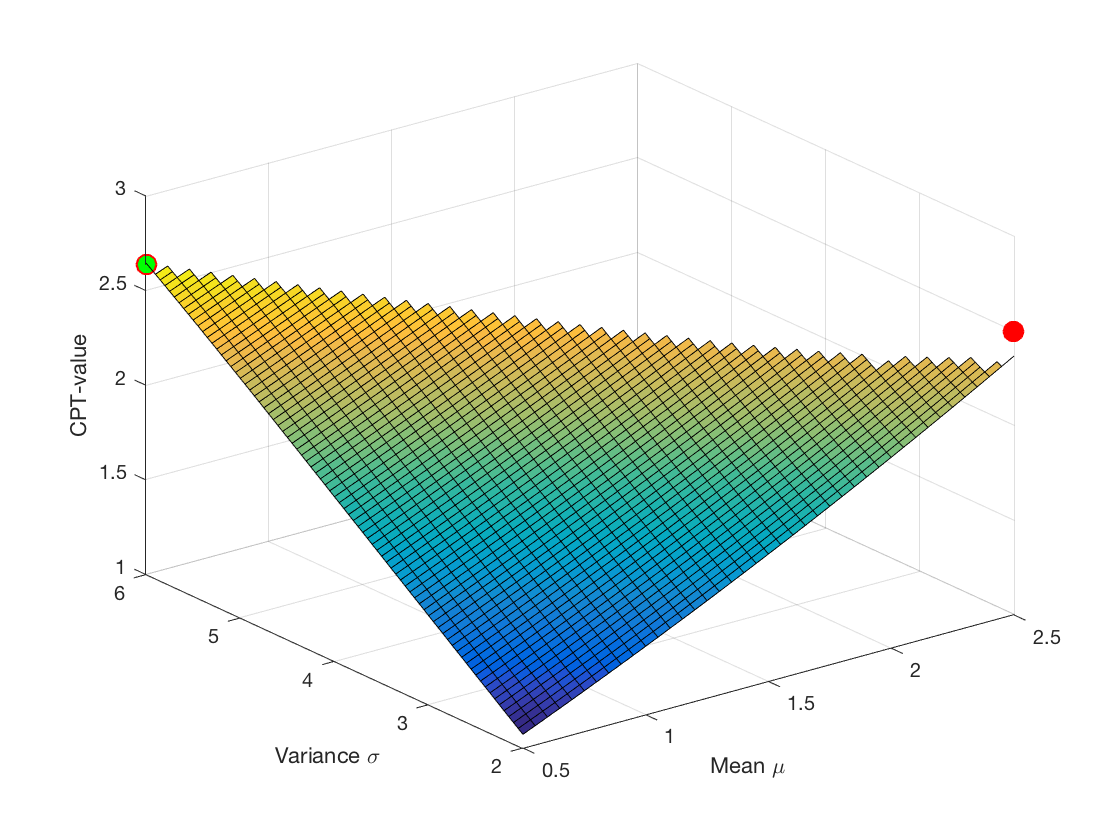
\includegraphics[width=3.5in]{fig/CPT_Normal.png}
   }
   }
  \caption{CPT-value of normal distributed r.v.s with parameters mean $\mu$ and variance $\sigma$. The red and green dots indicate the expected and CPT-value optima, respectively.}
   \label{fig:normal-cpt}
  \end{minipage}
%%%%%%%%%%%%%%%%%%%%%%%%%%%%%%%%%%%%%%%
\begin{minipage}{.01\textwidth}
~ 
\end{minipage}
%%%%%%%%%%%%%%%%%%%%%%%%%%%%%%%%%%%%%%%
   \begin{minipage}{.6\textwidth}
      \begin{tabular}{cc}
\subfigure
   {
%    \label{fig:skewnormal-expected}
   \scalebox{0.6}{
   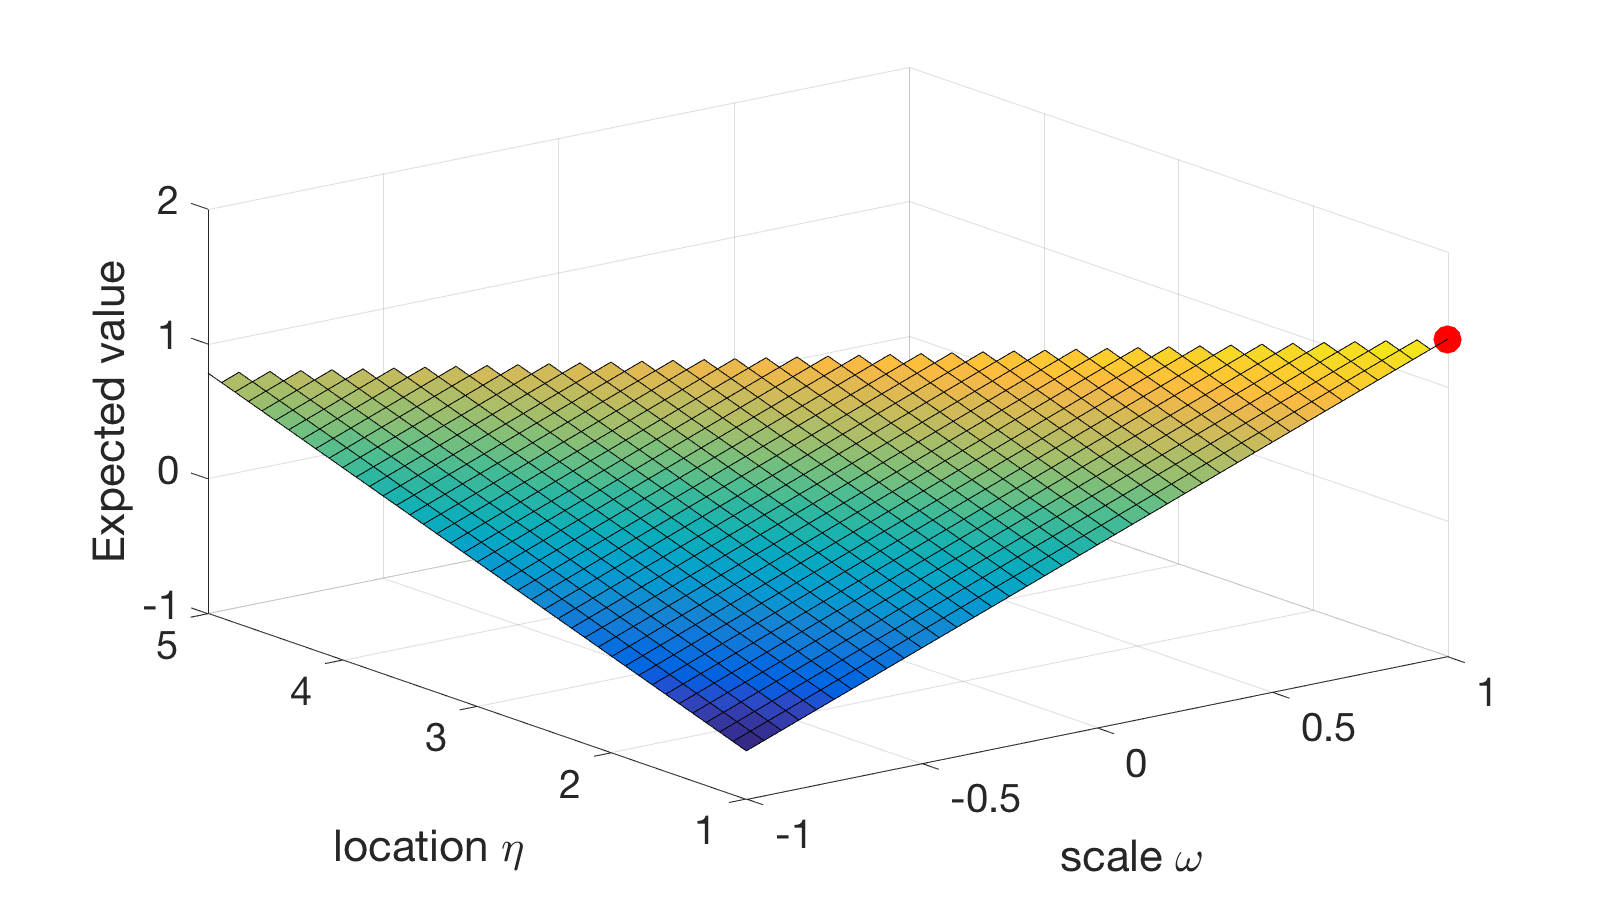
\includegraphics[width=3.5in]{fig/Expectation_skewNormal.png}
   }
   }
   &
\subfigure
   {
%    \label{fig:skewnormal-cpt}
   \scalebox{0.6}{
   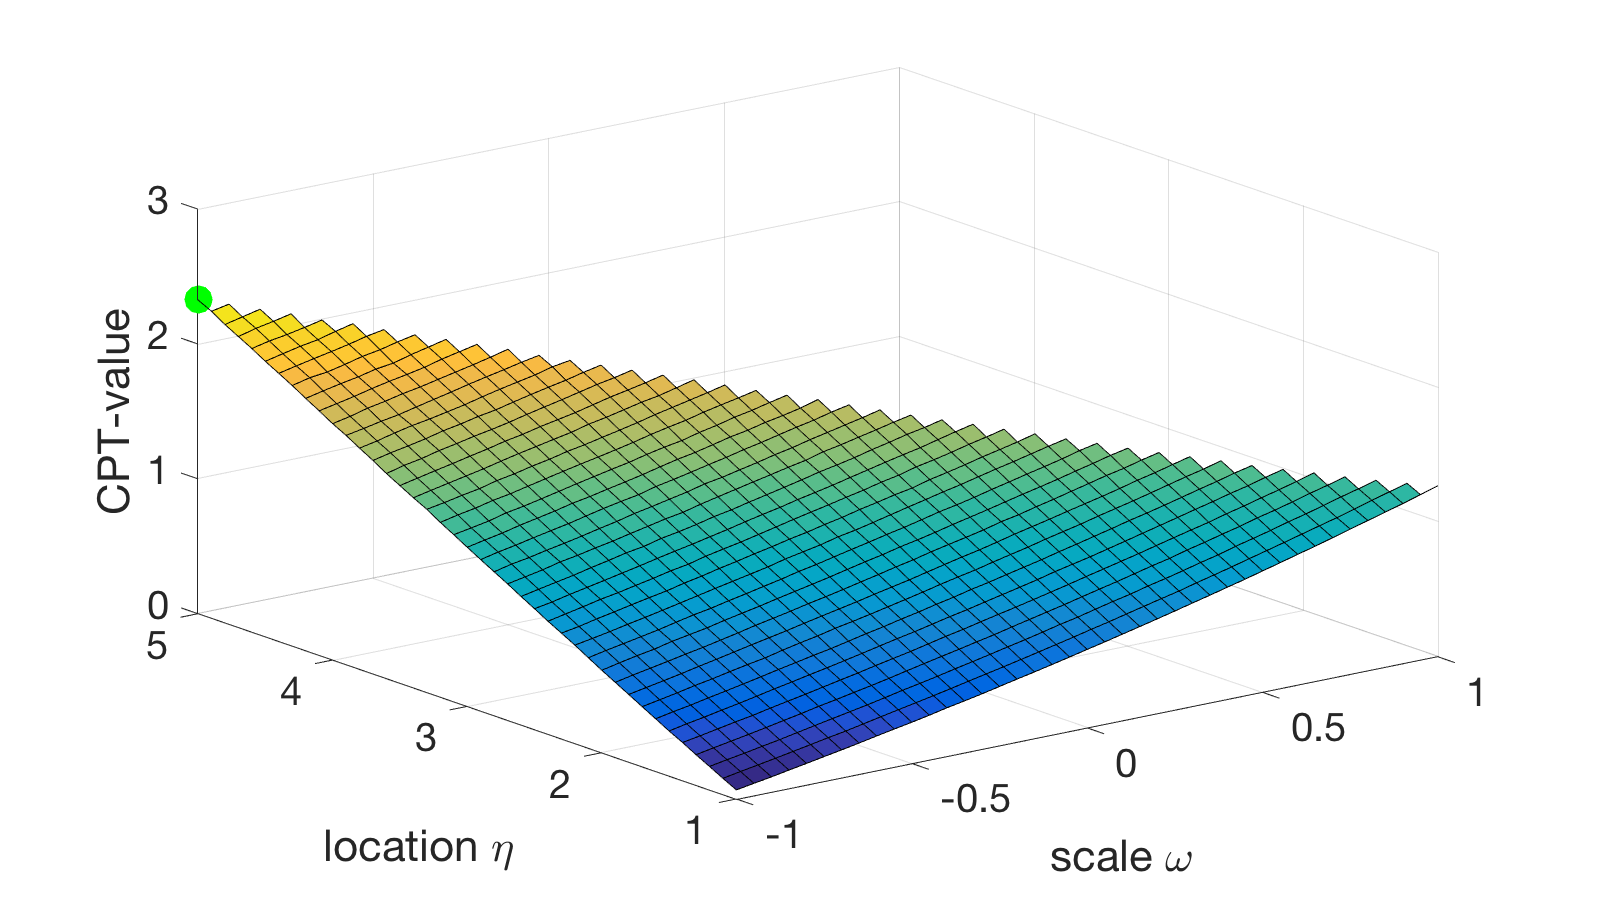
\includegraphics[width=3.5in]{fig/CPT_skewNormal.png}
   }
   }
   \end{tabular}
\caption{Expected and CPT values of skewed normal distributed r.v.s with fixed shape $\alpha=0.5$ and varying location $\xi$ and scale $\omega$. The red and green dots indicate the expected and CPT-value optima, respectively.}
\label{fig:skewnormal}
\end{minipage}

% \caption{Optimal expected and CPT-values within the feasible region (shaded green) for two different distributions.}
% \label{fig:cpt-synthetic}
\end{figure*}
\begin{example}
We consider normal distributed r.v.s with mean $\mu$ and variance $\sigma$. As shown in Figure \ref{fig:normal-cpt}, the feasible region for $(\mu, \sigma)$ is the triangle with vertices $(0.5,2), (0.5,6)$ and $(2.5,2)$. The expected value takes its maximum at $(2.5, 2)$, while a numerical optimization of the CPT-value returned a maximum at $(0.5, 6)$, with corresponding CPT-value $2.65$. On the other hand, the CPT value of the r.v. $N(2.5, 2)$ was $2.37$.
\end{example}

\begin{example}
Here we consider skew normal distributed r.v.s $sn(\xi, \omega, \alpha)$ with location $\xi$, scale $\omega$ and shape $\alpha$.  
The mean of $X_{(\xi, \omega, \alpha)} \sim sn(\xi, \omega, \alpha)$ equals 
$\xi + \omega \delta \sqrt{\frac{2}{\pi}}$, while the  variance is
$\omega^2(1 - \frac{2\delta^2}{\pi})$, with $\delta = \frac{\alpha}{1 + \alpha^2}$.
We set $\alpha=0.5$ and set up the feasible region for parameters $(\xi, \omega)$ to be the triangle with vertices $(-1,1), (1,1)$ and $(-1,5)$ as shown in Figure \ref{fig:skewnormal}.  
It turns out that the point $(-1,5)$ returns the largest CPT-value, with $\C(X_{-1,5,0.5,0.5}) = 2.30$, while
$\mathbb{E}(X_{-1,5,0.5}) = 0.78$.
On the other hand, the point $(1,1)$ has the largest expected value with $\mathbb{E}(X_{1,1,0.5}) = 1.36$, but the CPT value of the same r.v. is $1.25$.
\end{example}

%Our second example is concerned with skew normal distribution, 
%$sn(\xi, \omega, \alpha)$, where the mean equals 
%$\xi + \omega \delta \sqrt{\frac{2}{\pi}}$, and variance equals 
%$\omega^2(1 - \frac{2\delta^2}{\pi})$, with $\delta = \frac{\alpha}{1 + \alpha^2}$.
%We decide to work on 21 r.v.s as well, denoted as $Y_i \sim sn(\xi_i, \omega_i, \alpha_i)$.
%We will vary $\xi$ from $0$ to $2$ with ascending order and evenly gap, and vary $\omega$ from $5$ to $1$ with descending order with evenly gap. 
%The table \ref{tab:skewNormalCPT} exemplifies that the optimal-points of CPT-functional and expectation are very distinct as well. 

%\subsection{Consistency of CPT estimator}
We illustrate that the estimator in Algorithm \ref{alg:holder-est} converges rapidly by considering a skew normal distributed  r.v. $X$ with location, scale and shape parameters set to $2,1$ and $2$, respectively. For calculating the CPT-value, we use the trapezoidal rule. 
We conduct the experiment in $100$ simulation phases indexed from $1$ to $100$. In each phase $i$, we generate i.i.d. estimators $\overline\C^j_{n_i}\left(X\right)$ using Algorithm \ref{alg:holder-est} and $n_i$ samples of skew normal distributed r.v. $X$, where $j=1,\ldots,10$ corresponds to an independent simulation. The number of samples $n_i$ in each phase $i$ ranges from $100$ to $10^6$. For each phase $i$ that corresponds to $n_i$ samples, we calculate the deviation of the estimator $\overline \C_{n_i} = \frac1{10}\sum_{j=1}^{10}\C^j_{n_i}$ from the numerically integrated CPT-value. Figure \ref{fig:cpt-est} presents the mean and standard error for each $n_i$. 
% Here, the margin of error denotes half the length of t-confidence interval. 
It is evident from Figure \ref{fig:cpt-est} that our CPT-value estimate gets very close to the true CPT-value rapidly.

%%%%%%%%%%%%%%%%%%%%%%%%%%%%%%%%%%5
%%%% Error bars 
%%%%%%%%%%%%%%%%%%%%%%%%%%%%%%%%%%%%
\newcommand{\errorband}[5][]{ % x column, y column, error column, optional argument for setting style of the area plot
\pgfplotstableread[col sep=tab, skip first n=2]{#2}\datatable
    % Lower bound (invisible plot)
%     \addplot [draw=none, stack plots=y, forget plot] table [
%         x={#3},
%         y expr=\thisrow{#4}-2*\thisrow{#5}
%     ] {\datatable};

    % Stack twice the error, draw as area plot
    \addplot [draw=none, fill=gray!40, stack plots=y, area legend, #1] table [
        x={#3},
        y expr=4*\thisrow{#5}
    ] {\datatable} \closedcycle;

    % Reset stack using invisible plot
    \addplot [forget plot, stack plots=y,draw=none] table [x={#3}, y expr=-(\thisrow{#4}+2*\thisrow{#5})] {\datatable};
}

\begin{figure}
    \centering
\scalebox{0.7}{\begin{tikzpicture}
      \begin{axis}[
	xlabel={Sample size $n_i$},
	ylabel={Estimation error $|\overline \C_{n_i} - \tilde \C(X)|$},
       %legend entries={
	 %,
        %estimator,
        %},
        %legend pos=north east,
				grid,grid style={gray!30}
      ]

      \errorband[red!50!white, opacity=0.3]{results/estimation_accuracy.txt}{0}{1}{2}
      \addplot [thick, red] table [x index=0, y index=1,col sep=tab] {results/estimation_accuracy.txt};
      \end{axis}
      \end{tikzpicture}}
			\caption{Difference between CPT-estimate $\overline \C_{n_i}$ using Algorithm \ref{alg:holder-est} and numerically integrated approximation $\tilde \C(X)$ to CPT-value $\C(X)$ of a skew normal distributed r.v. $X$ with shape $2$, location $2$ and scale $1$. The shaded bands denote the standard error calculated from ten independent simulations.  }
      \label{fig:cpt-est} 
			\end{figure}
